\section{Replication of Published Results}
\label{sec:replication}
Each published result was rebuilt from its description, run independently and compared with what the source states; no source code was available. \nb{A result counts as \emph{reproduced} only when a stated number or functional form is matched within the stated tolerance, and nothing was tuned to improve agreement. \Cref{fig:scorecard} compares our values with the published or theoretical ones and \cref{tab:replication} classifies each replication; \cref{fig:repl} shows the comparisons themselves.}

\begin{figure*}[t]
\centering
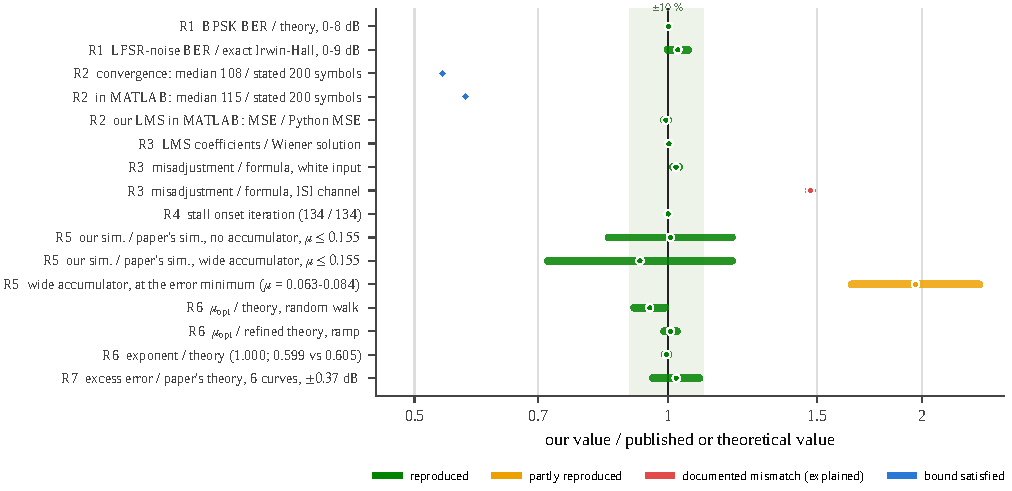
\includegraphics[width=0.8\linewidth]{figs/scorecard.pdf}
\caption{\nb{Replication scorecard: our value divided by the published or theoretical value (bars: range over the stated conditions; shaded: $\pm10$\,\%). Most reproduced results lie inside $\pm10$\,\%; the R5 bands are wider because they include about $\pm5$\,\% digitising error of the paper's points. The R3 ISI point is the documented misadjustment mismatch, explained in \cref{sec:misadj}; R2 is an upper bound (``less than 200 symbols''), satisfied with margin by our model and by MATLAB; MathWorks' LMS run on our own samples agrees with our model within 1.2\,\%.}}
\label{fig:scorecard}
\end{figure*}

\textbf{R1 --- BPSK in AWGN.} The flat-channel error rate is $Q(\sqrt{2E_b/N_0})$ \cite{proakis2008}. \nb{Simulated BER / theory is 1.000--1.002 for 0--8\,dB ($2\times10^7$ symbols) and 0.95/0.92 at 9/10\,dB with 639/71 errors, statistically consistent. For the 12-uniform hardware noise, the exact Irwin--Hall BER \cite{irwin1927,hall1927} is matched to 0.998--1.056 (\cref{fig:repl}a).}

\textbf{R2 --- MathWorks ``Equalize a BPSK signal''} \cite{mathworks}: an 8-tap LMS equalizer, step 0.1, channel $[0.02+0.5j,\ 0.05]$, 30\,dB, 200 training symbols; the page states that the equalizer ``converges in less than 200 bits''. \nb{Our re-implementation converges at a median of 108 symbols (5--95\,\%: 97--123), 1000/1000 runs within 200, with no post-training errors (\cref{fig:repl}b). Assumed, because the page does not state them: the complex LMS convention and the initial weights; both initialisations give the same result. This channel is nearly ISI-free after derotation, so the example tests convergence, not ISI removal. The original example was also run in MATLAB R2025b with MathWorks's own equalizer (\texttt{comm.LinearEqualizer}, 1000 runs): median 115 symbols (5--95\,\%: 103--133), 1000/1000 runs under 200 symbols and 1000/1000 without post-training errors. The two medians differ by about 7 symbols (6\,\%), plausibly through MATLAB's initial weights and alignment convention, which the page does not state; the published claim is confirmed by both.}

\nb{\emph{MATLAB cross-check of our own LMS model.} On our received samples (primary channel at $c=40$ and $c=116$, 14\,dB, 16 taps, $\mu=2^{-8}$), MathWorks' LMS equalizer gives a steady-state MSE of 0.022449 and 0.055030 against our 0.022469 and 0.055690 (ratios 0.999 and 0.988, at its best reference tap), and the same LMS equations written as a plain MATLAB loop reproduce our MSE and final coefficients to every printed digit (ratio 1.00000). The Python model is therefore confirmed by an independent tool (\lvl{L1}).}

\textbf{R3 --- stationary LMS theory.} LMS converges to the Wiener filter and its misadjustment is about $\mu\,\mathrm{tr}(\mathbf R)/2$ \cite{widrow1976,haykin2014}. \nb{Convergence to the Wiener filter (coefficients within 0.17--0.18\,\%) and the misadjustment formula on a white-input control (within 1--3\,\%) are reproduced. On the ISI channel the measured excess is 1.47--1.48 times the formula; this documented mismatch is explained in \cref{sec:misadj}.}

\nb{\textbf{R4 --- stall onset} \cite{shahdoosti2018}: AR(10) signal with the paper's initial values, $\mu=0.01$, 12 fractional bits, rounding. The paper reports that stalling begins at iteration 134, with the threshold $e_T=\mathrm{LSB}/(2\mu u)=0.0244$ for $u=0.5$. Our first iteration with all updates rounded to zero is \textbf{134} (\cref{fig:repl}c). The paper does not state how the desired signal is formed; one-step prediction was assumed. With truncation instead of rounding the onset is 129--130, so the agreement depends on the rounding rule that the paper states.}

\nb{\textbf{R5 --- fixed-point steady-state error} \cite{ghanassi2007} (read in full): $N=100$ taps, 16 bits, white Gaussian input of variance 0.1, $\|\mathbf w_o\|^2=0.4$, no noise, with and without a wide accumulator. An earlier rebuild, made from a partly unreadable copy, rounded the update $\mu e\mathbf u$ once; the full text shows two quantisers, first $Q[\mu e]$ and then $Q[Q[\mu e]\,u]$ (its Eqs.~5b, 17). The rebuild was corrected and nothing else changed, then run at the paper's own step sizes and compared with the paper's \emph{simulation} points, digitised from its Figs.~2 and 3 (reading error about $\pm5$\,\%). For $\mu\le0.155$ our steady-state error is 0.85--1.19 times the paper's at all 18 points without accumulator, and 0.72--1.19 times at 15 of 18 points with it (\cref{fig:repl}d). The exceptions are the narrow error minimum of the accumulator variant ($\mu=0.063$--0.084, 1.65--2.34 times), where the error is only a few times the quantisation floor, and the last points before the stability limit $\mu<0.2$ ($\mu\ge0.169$), where the error rises steeply and a small difference in $\mu$ changes it by orders of magnitude. The paper's \emph{formulas}, by contrast, match both its own points and ours only in parts: the stall law within 0.70--0.97, the intermediate formula within about 1.3 without accumulator, the stochastic-gradient formula within 0.54--0.86. That gap lies between the paper's analysis and its own experiment, not in our rebuild. One modelling choice was made after seeing a result: building the reference from the unquantised input adds a $10^{-5}$ floor from rare input saturation, absent from the paper's results, so the quantised reference was used. \emph{Reproduced (the paper's simulation), with the two stated exceptions.}}

\textbf{R6 --- the tracking trade-off \eqref{eq:mis}} \cite{widrow1976,haykin2014,macchi1995}\nb{, with the deterministic-drift form of \cite{vlaski2020,bershad1989}: system identification with 8 taps, white input, and a random-walk or deterministic-ramp optimum (\cref{fig:repl}e). The lag slopes $-1$ (random walk) and $-2.01$ (ramp) and the gradient-noise slope $+1$ are reproduced; $\mu_{\rm opt}$ agrees with \eqref{eq:mis} within 1--9\,\% and the measured random-walk exponent is 1.000. For the ramp the exponent is 0.60 instead of the first-order 2/3, because the optimum moves to large $\mu$ where the first-order gradient-noise term is too small; with the exact white-input term the theory gives 0.605 and the optimum agrees within 1--2.4\,\%. This is the same finite-step effect found on our own channel (\cref{sec:theory}).}

\nb{\textbf{R7 --- LMS tracking of gain variations} \cite{bergmans1990} (read in full): LMS identification of a 5-tap channel $f_0=1$, $f_2=-1$ whose output is scaled by $1+g_k$, with $g_k$ a first-order autoregressive (low-pass) gain of bandwidth $\beta$; binary input, Gaussian noise, $c_0=f$, 16384 samples per $\mu$. The paper derives the excess error as gradient noise (its Eq.~10) plus a lag error (its Eq.~27), predicts from its Eq.~32 whether the total error rises monotonically with $\mu$ or has a minimum, and reports simulation within about $\pm0.2$\,dB of theory in its Figs.~2--4. All six curves of those figures were rebuilt (20 runs per point). Our simulation lies within $-0.18$ to $+0.14$\,dB of the theory on four curves and within $+0.23$ and $+0.37$\,dB on the two with $\beta=0.1$ at 25\,dB and at 5\,\% gain variation, in the middle range of $\mu$ (\cref{fig:repl}f). The monotone/minimum classification of Eq.~32 is confirmed on all six curves; the minimum is 2.4\,dB deep at 5\,\% (theory 2.6\,dB), 1.35\,dB at 25\,dB (theory 1.5\,dB) and only 0.1\,dB at 20\,dB, 2\,\%, where its position is not resolvable. The residual excess disappears (all curves within $\pm0.18$\,dB) when the lag error is also counted as a driver of gradient noise ($N_0\to N_0+\varepsilon_l$ in Eq.~10); this is a diagnostic, not a change to the verdict, and it is the same mechanism as our misadjustment correction (\cref{sec:misadj}): an error that the filter cannot remove adds to the gradient noise. \emph{Reproduced}, with a slightly larger deviation than the stated $\pm0.2$\,dB on two curves.}


\begin{table}[t]
\centering\small
\caption{\nb{Replications by type. Levels: R1--R3, R6 and R7 \lvl{L1}; R4 and R5 are small stand-alone fixed-point models, not the project's \lvl{L2}.}}
\label{tab:replication}
\color{blue}
\setlength{\tabcolsep}{3pt}
\begin{tabular}{@{}lp{0.47\linewidth}p{0.36\linewidth}@{}}
\toprule
& Quantity & Type of replication\\
\midrule
R1 & BPSK BER; exact BER of the LFSR noise & exact (numerical)\\
R2 & MathWorks example, convergence $<200$ & qualitative (bound); confirmed in MATLAB\\
R3 & Wiener convergence; misadjustment & exact on white input; mismatch on ISI, explained\\
R4 & stall onset at iteration 134 & exact\\
R5 & fixed-point steady-state error & paper's simulation reproduced, except at the accumulator minimum and near instability; its formulas only partly\\
R6 & lag/noise trade-off, $\mu_{\rm opt}$ scaling & exact (functional form)\\
R7 & excess error with gain variations; monotone or minimum & functional form, within $\pm0.37$\,dB; classification exact\\
\bottomrule
\end{tabular}
\end{table}

\begin{figure*}[t]
\centering
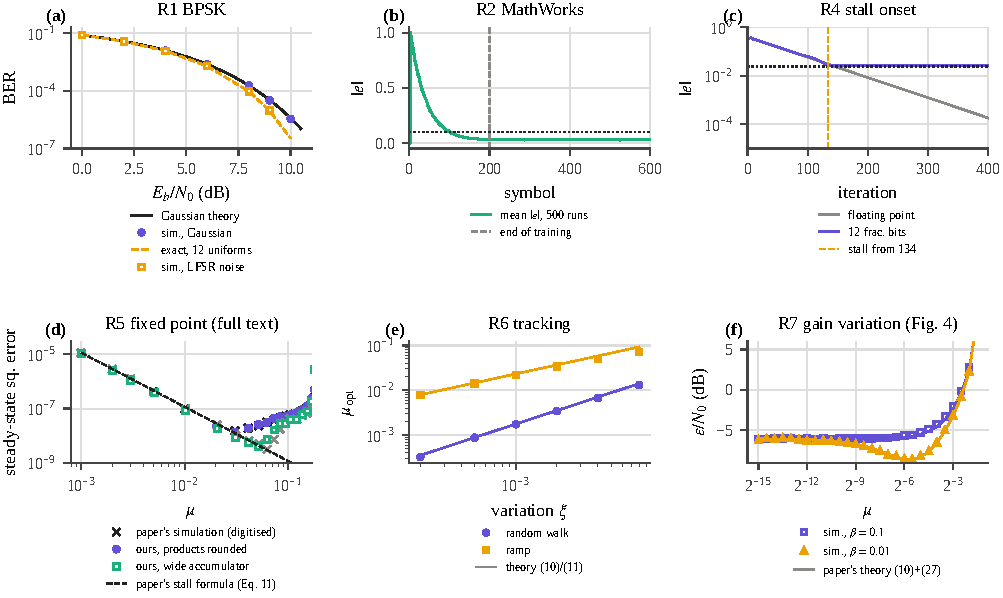
\includegraphics[width=\linewidth]{figs/replication.pdf}
\caption{\nb{Replications (\lvl{L1}; R4, R5 stand-alone fixed-point models). (a)~R1: BPSK BER against Gaussian theory, and the LFSR (12-uniform) noise against its exact Irwin--Hall BER. (b)~R2: mean error magnitude of the MathWorks 8-tap equalizer over 500 runs; it falls below 0.1 at about 100 symbols, inside the 200-symbol training. (c)~R4: error magnitude of fixed-point LMS; every update rounds to zero from iteration 134, as published, while floating point keeps converging. (d)~R5, rerun after reading the full text: our steady-state error and the paper's own simulation points at the same step sizes, with its stall formula \cite{ghanassi2007}. (e)~R6: optimum step against the variation for a random-walk and a ramp optimum, with theory; the ramp departs at large $\mu$ (finite-step effect). (f)~R7: excess error against step size for the case of Fig.~4 of \cite{bergmans1990} (20\,dB, 5\,\% rms gain variation), with the paper's theory; the narrow-band gain ($\beta=0.01$) gives a minimum, the wide-band one ($\beta=0.1$) a monotone rise.}}
\label{fig:repl}
\end{figure*}
